\documentclass[11pt,a4paper]{article}
\usepackage[margin=1in]{geometry}
\usepackage{graphicx}
\usepackage{hyperref}
\usepackage{csquotes}
\usepackage[backend=bibtex,style=authoryear]{biblatex}
\addbibresource{refs.bib}

\title{Veni Alea}
\author{Julian Hammerton}
\date{\today}

\begin{document}
\maketitle

\vspace{1em}
\begin{center}
  {\small © 2025 Julian Hammerton. All rights reserved.}
\end{center}

\section{Introduction}
Hello, world. See Fig.~\ref{fig:example}. For references, see \textcite{knuth1984texbook}.

\begin{figure}[h]
  \centering
  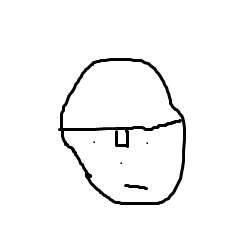
\includegraphics[width=.5\linewidth]{figures/example.png}
  \caption{An example figure.}
  \label{fig:example}
\end{figure}

\printbibliography
\end{document}